\usemintedstyle{manni}

\section{Intro}

%Content:
% - Difference asynchronously, parallel
% - Explanation Coroutines
% - asyn function, await function in example
% - introduction to examples (moving all blocking calls out)

\begin{frame}[fragile]
	\frametitle{Toolchain}
	\begin{itemize}
		\item LLVM/Clang 6.0
		\item Linux
	\end{itemize}
\end{frame}

\newcommand{\code}[4]{\inputminted[fontsize=\scriptsize,firstline=#1,lastline=#2,xleftmargin=#3]{cpp}{../mixed/src/#4}}

\begin{frame}[fragile]
	\frametitle{Todays Subject}
	\code{12}{16}{10pt}{sync/http_client.h}
\end{frame}


\section{Examples}

\newcommand{\simpleexample}[7]{%
	API
	\code{#6}{#7}{0pt}{#5/http_client.h}
	\vspace{1mm}
	%\pause
	Callee
	\code{#1}{#2}{0pt}{presentation_examples_test.h}
	\vspace{1mm}
	%\pause
	Caller
	\code{#3}{#4}{-16pt}{presentation_examples_test.cpp}
}

\begin{frame}{[fragile]}
	\frametitle{Plain call}
	\simpleexample{22}{26}{15}{16}{sync}{12}{16}
	\begin{itemize}
		\item What if I don't want to block during the request\_get?
	\end{itemize}
\end{frame}%

\begin{frame}{[fragile]}
	\frametitle{std::thread}
	\simpleexample{30}{39}{22}{23}{threaded}{12}{16}
\end{frame}%

\begin{frame}{[fragile]}
	\frametitle{std:.async blocking}
	\simpleexample{41}{49}{29}{30}{threaded}{12}{16}
\end{frame}%

\begin{frame}{[fragile]}
	\frametitle{std::async non-blocking}
	\simpleexample{51}{56}{36}{38}{threaded}{12}{16}
\end{frame}%

\begin{frame}[fragile]
	\frametitle{Motivation}
	\begin{figure}[ht]
		\centering
		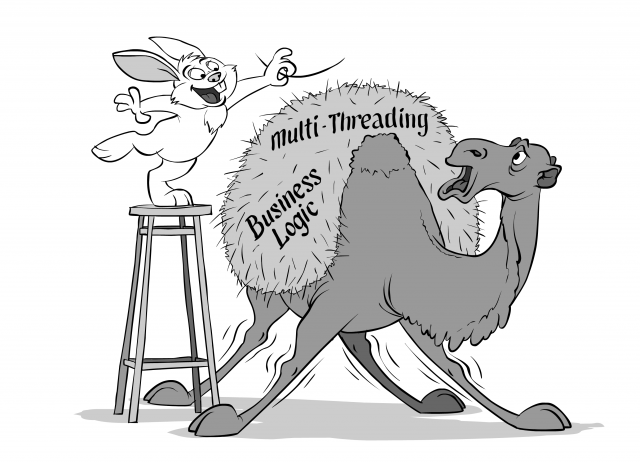
\includegraphics[width=0.6\textwidth]{img/multi-threading}\\
		{\tiny http://ithare.com/}\\
	\end{figure}
	\vspace{5mm}
	What have we got now?
	\begin{itemize}
		\item uncontrolled creation and destruction of threads
		\item is this maintainable?
	\end{itemize}
\end{frame}

\begin{frame}[fragile]
	\frametitle{Sequential, Concurrent, Parallel}
	\begin{figure}[ht]
		\centering
		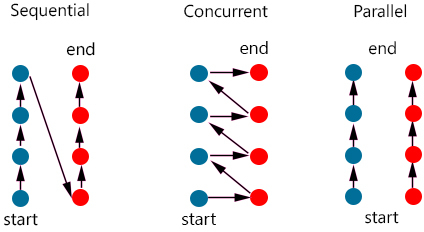
\includegraphics[width=0.8\textwidth]{img/parallel_sequential_concurrent}\\
		{\tiny http://www.dietergalea.com/parallelism-concurrency/}\\
	\end{figure}
	\vspace{5mm}
	We wanted concurrent processing, but we introduced parallelism now
\end{frame}

\begin{frame}[fragile]
	\frametitle{Executor}
	\inputminted[fontsize=\scriptsize,firstline=12,lastline=35]{cpp}{../mixed/src/executor.h}
\end{frame}

\begin{frame}{[fragile]}
	\frametitle{Callbacks}
	\simpleexample{61}{65}{44}{47}{callback}{12}{18}
	\pause
	\begin{itemize}
		\item Composability?
	\end{itemize}
\end{frame}%

\begin{frame}[fragile]
	\frametitle{Encapsulate callbacks $\rightarrow$ Task}
	Callbacks are not composable in a sane way, so we introduce a task, which should behave like this:
	\vspace{3mm}
	\begin{minted}[fontsize=\scriptsize]{cpp}
    template <typename T>
    struct task_t { 
      task<...> then(auto continuation);
      void set_result(T result);
    };
    template <typename T> using task = std::shared_ptr<task_t<T>>;
    task<std::tuple<...>> when_all(task, ...);

    //example:
    task<int> first__task = get_number();
    task<int> second_task = get_number();
    when_all(first_task, second_task)->then(
      [](std::tuple<int, int> values) {
        return std::get<0>(first) + std::get<1>(second);
      })->then([](int sum) {
        std::cerr << sum << std::endl;
      })->then([]{
        //after cerr
      });
  \end{minted}
\end{frame}

\begin{frame}{[fragile]}
	\frametitle{Tasks }
	\simpleexample{76}{82}{62}{65}{task}{13}{17}
\end{frame}%

\begin{frame}{[fragile]}
	\frametitle{Coroutines}
	\begin{figure}[ht]
		\centering
		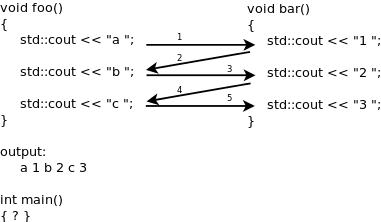
\includegraphics[width=0.6\textwidth]{img/foo_bar}\\
		{\tiny https://www.boost.org/doc/libs/1\_67\_0/libs/coroutine/doc/html/coroutine/intro.html}\\
	\end{figure}

	A Coroutine is a \textbf{normal function}, which in addition to be able to be \textbf{called} and having a \textbf{return value}:
	\begin{itemize}
		\item can be suspended (return the control to the caller), which is usually called yield or await
		\item and resumed (return the control back to the coroutine)
	\end{itemize}
	Basically, it allows implementing cooperative multitasking in a readable way
\end{frame}%

\begin{frame}[fragile]
	\frametitle{Async and await on top of  in Boost.Coroutine2}
	On top of Boost.Coroutine2, which implements a generic stackful coroutine system, the following functions can be implemented:
	\begin{minted}[fontsize=\scriptsize]{cpp}
    //start an async operation (start the coroutine)
    template <typename Fn>
    task<...> async(Fn fn);

    struct Await {
      //wait for an async operation to complete (suspend the coroutine)
      template <typename T>
      T operator()(task<T> task);
    };

    they can be used as follows:
    task<void> task = async([](Await await) {
      await(long_running_async_task());
      //do something synchronously
      await(some_other_task());
    });
    task->then([]{
      // gets here when the coroutine completes
    });
  \end{minted}
\end{frame}


\begin{frame}{[fragile]}
	\frametitle{Task with Boost.Coroutines2}
	\simpleexample{87}{93}{71}{74}{boost_coroutine}{87}{90}
\end{frame}%
\begin{frame}{[fragile]}
	\frametitle{Task with coroutines-ts}
	\simpleexample{105}{109}{89}{92}{coroutine_ts}{95}{99}
\end{frame}%

\begin{frame}[fragile]
	\frametitle{From sequential to coroutine}
	Sequential Blocking Style
	\code{22}{26}{8pt}{presentation_examples_test.h}
	\vspace{8mm}
	Asynchronous non-blocking Style (likely C++20)
	\code{105}{109}{8pt}{presentation_examples_test.h}
	\vspace{8mm}

	Where is the difference now?
\end{frame}

\section{Hands On}
\begin{frame}[fragile]
	\frametitle{Hands On}

	{\large Given}
	\inputminted[fontsize=\scriptsize,firstline=6]{cpp}{../dojo/first/http_client.h}
	\inputminted[fontsize=\scriptsize,firstline=12,lastline=16]{cpp}{../dojo/first/sync/http_client.h}
	\vspace{5mm}
	{\large To implement}
	\inputminted[fontsize=\scriptsize,firstline=18,lastline=20]{cpp}{../dojo/first/sync/http_client.h}
\end{frame}
